% Marius-Juston 2026
\documentclass[tikz,border=10pt]{standalone}
\usepackage{tikz}
\usetikzlibrary{shapes.geometric, arrows.meta, positioning, calc}


\begin{document}


    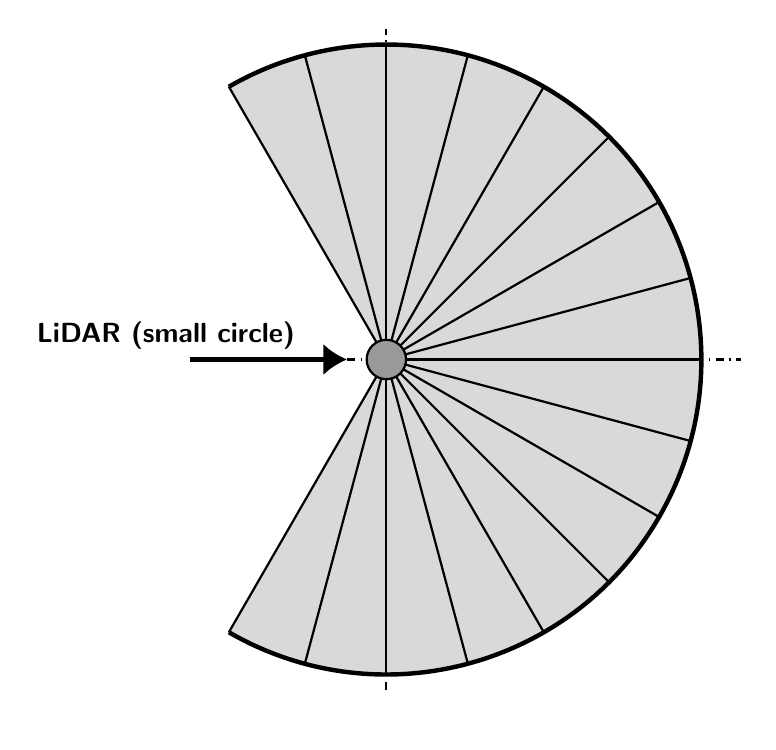
\begin{tikzpicture}

    % Define parameters for easy adjustment
    \def\radius{4cm}          % Outer radius of the sector
    \def\startAngle{-120}     % Starting angle (bottom left)
    \def\endAngle{120}       % Ending angle (top left)
    \def\numSectors{16}       % Number of wedges
    \def\innerRadius{0.25cm}  % Radius of the central LiDAR circle

    % 1. Draw the filled background sector
    \fill[gray!30] (0,0) -- (\startAngle:\radius) arc (\startAngle:\endAngle:\radius) -- cycle;

    % 2. Draw the radial lines (the dividers)
    \foreach \i in {0,1,...,\numSectors} {
        \pgfmathsetmacro{\currentAngle}{\startAngle + \i * (\endAngle - \startAngle) / \numSectors}
        \draw[thick] (0,0) -- (\currentAngle:\radius);
    }

    % 3. Draw the outer arc boundary
    \draw[ultra thick] (\startAngle:\radius) arc (\startAngle:\endAngle:\radius);

    % 4. Draw the dashed symmetry lines (Horizontal and Vertical)
    \draw[dash dot, thick] (-0.5,0) -- (\radius+0.5cm, 0); % Horizontal axis
    \draw[dash dot, thick] (0, -\radius-0.2cm) -- (0, \radius+0.2cm); % Vertical axis

    % 5. Draw the central LiDAR unit (the small circle)
    \draw[fill=gray!80, thick] (0,0) circle (\innerRadius);

    % 6. Add the Arrow and Text Label
    \draw[line width=1.5pt, -{Latex[length=3mm, width=4mm]}] (-2.5,0) -- (-0.5,0);
    \node[anchor=south, align=center, font=\sffamily\bfseries] at (-2.8,0) {LiDAR (small circle)};
\end{tikzpicture}


\end{document}